\section{Forwards-engineered Childbirth Simulation}\label{methodology-basic}

\subsection{Physics based simulation}

  \subsubsection{Simplified physics models}

  There are different levels of complexity at which a physics model can be formulated. The same physical concept can be represented with a higher or lower degree of simplified approximation.

  Physics based simulations find a great number of applications in various areas. Not all such areas require highest fidelity models. Games and entertainment industry is an exmaple of areas where a simplified model yeilds sufficiently accurate results with a relatively cheap cost of the computation required.

  \subsubsection{Simplifying assumptions}

  The intial attempts on creating a forwards-engineered simulation of human childbirth were focused on using simplied physics model. Due to the requirement on having a childbirth simulation working as soon as possible, a list of simplifying assumtions was adopted.

  The list included the following assumtions:

  \begin{enumerate}

    \item The soft tissues of the maternal reproductive system do not need to be considered to observe cardinal movements
    \item The trunk of the fetal body does not need to be considered to observe cardinal movements.
    \item The labour forces can be replaced by a simple periodical force acting on the atlanto-occipital point (Figure \ref{ao-point}) of the fetal skull to observe cardinal movements.

  \end{enumerate}

  \begin{figure}
  \begin{center}
  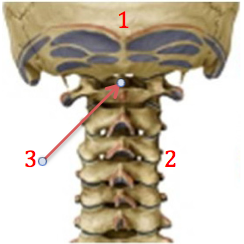
\includegraphics[width=40mm]{sections/methodology/images/basic/ao-point.png}
  \caption[The atlanto-occipital point.]{\label{contact} The atlanto-occipital point.}
  \end{center}
  \end{figure}

  The assumtions allowed for a simpler set of requirements for the software implementation aspect of the project and arriving at a working prototype soon.


\subsection{IveTrainer childbirth simulation software}

\subsubsection{Overview}

The IveTrainer software was the first attempt on implementing a forward-engineered childbirth simulation. It was limited to the simplified physics model described above.

The resulting software is a simulation tool capable of performing several different simulations. The set of simulations can be extended easily because of the software design pattern utilisation. The simulations can be run in the fully forward engineered mode or using imposed trajectories and fetal postures in a reverse engineered way. It provides several input modalities, namely: keyboard, mouse and haptic device.

The use of reverse engineering was justified as the chosen forward engineering approach failed to give sufficiently accurate results. However, as mentioned in the Literature Review \ref{lit-existing}, many of contemporary simulation systems use reverse engineering. Additionally, the two forward and reverse engineered approaches were combined, resulting in a hybrid simulation partially dictated by a predefined trajectory and partially by the underlying physics simulation. Figure \ref{hybridFig} shows the difference between the fully reverse-engineered and the hybrid approach.

\begin{figure}
  \centering
    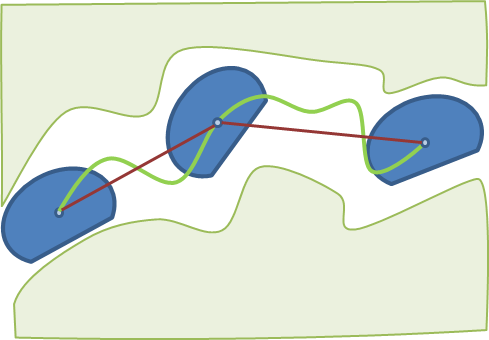
\includegraphics[width=60mm]{sections/methodology/images/basic/hybrid-trajectory.png}
  \caption[The reverse-engineered trajectory in red and the hybrid trajectory in green.]{\label{hybridFig} The reverse-engineered trajectory in red and the hybrid trajectory in green. It can be seen that the head passes through the specified way-points, but also interacts with passage walls.}
\end{figure}

Currently, each simulation consists of three objects and a simulation procedure that defines what interactions between the objects are to be simulated. The three objects are: a fetus, a pelvis and a user controlled hand. In the first simulation, the fetus is represented by its head alone, whereas in the second the full articulated fetal body is used. The pelvis is represented by a complex customizable model. The hand is controlled by the user using spatial 3D input from a connected haptic device.

\subsubsection{Features}

The set of features is currently comprised of means for child delivery simulation for predicting potential outcomes and delivery process visualisation for training purposes. The main features of the system in more detail are provided below.

\paragraph{Object Manipulation}
Object manipulation is a basic, but crucial feature of the system. Considering that the system is meant to be used by medical personal, a user-friendly interface for object manipulation was provided. Thus, the system is incorporated with the means of easy control over the objects' position and orientation using a mouse. This is achieved by implementing an \emph{arcball} input system and a set of keyboard shortcuts.

\paragraph{Cardinal Movements of Fetal Head}
The first simulation is dedicated to the simulation of cardinal movements of the fetal head only. Provided additional improvement of the underlying physical model and refinement of the set of considered influences, this mode can be used to analyse and investigate the childbirth process and eventually predict the most-likely outcome of a given vaginal delivery.


\paragraph{Customisable Models}
One of the most important features here is that the system provides a customizable environment. Namely, the main pelvimetric diameters and the diameters of the fetal head can be specified with sub-millimetric accuracy. This may have limited use in predicting real case outcomes, however, it can be used for the purposes of investigation of different child delivery processes.

The coronal, transverse and sagittal extents of the fetal head can be specified, to simulate and analyse how the given diameters affect the outcome of a given delivery. The set of customizable extents for the pelvis consists of the main obstetric diameters, namely: inlet transverse, inlet oblique, inlet anteroposterior, outlet transverse, outlet oblique, outlet anteroposterior and middle anteroposterior diameters. The illustration of all the described diameters will be given in the following sections.

\paragraph{Periodically changing expulsion force}
The control over expulsion force magnitudes and their temporal change is inspired by the work by \citet{Moreau}. The authors of this work indicated that the periodical nature of the forces cause the head to progress backwards through the birth canal as well forwards as it generally does. They suggested the potential importance of this phenomenon as an additional factor contributing to a successful delivery.

This idea was addressed while developing the software, by incorporating a sinusoidal signal generator. Given minimum and maximum magnitudes and a direction for the expulsion force, the generator can be used to interpolate between the minimum and maximum force magnitudes. The minimum force magnitude can be set to be negative, which allows the backwards propagation of the fetus.

\paragraph{Control over physical quantities}
The system allows the user to specify the essential physical quantities involved in the physics simulation. The most important ones include: minimal and maximal expulsion magnitudes, expulsion force change period and the friction coefficient. Each of the listed quantities can be set as required.

\paragraph{Imposed trajectory management}
The system is capable of forward-engineered simulation that extrapolates from the initial position based on the physical model and avoids any imposed characteristics. Along with this mode, the system can utilize predefined trajectories of the fetus, which specify the position, as well as the orientation, of the fetus for an arbitrary number of delivery stages.

The trajectory of the fetus consists of a set of stages. Each stage is a momentary snapshot of the fetal position and orientation at any given stage of the delivery. The snapshots are called \emph{way points} and are arranged into a list that forms a \emph{trajectory}.

The system allows convenient management of the trajectories by providing means to create, delete, edit, save and load them. Given a \emph{trajectory} consisting of several \emph{way points}, the user is able to create new and  remove, edit or rearrange existing ones.

\paragraph{Hybrid Simulation}
A compromise solution for the forward-backward engineered simulation was achieved. This implies that the simulation will proceed in the forward engineered mode, unless the simulated fetus deviates from the specified trajectory in terms of position and orientation. This allows current position and orientation to be optimized. Thus, using this approach the system can avoid cases when simulation leads to unrealistic outcomes.

\paragraph{Shoulder Dystocia Visualisation}
The second simulation is purely demonstrative visualisation of a shoulder dystocia case discussed in section \ref{dystociaSec}. It shows how the case occurs starting from the initial stages of labour till the state when the shoulder is pressed against the \emph{symphysis pubis}. The limitation of it is that the body of the baby is completely rigid.

\paragraph{Face Presentation}
One of the predefined trajectories demonstrates face presentation delivery. As expected the head will pass through the pelvis fully extended, but will be arrested near the outlet.

\paragraph{Manipulating Articulated Fetus}
The third simulation is a result of further development of the shoulder dystocia visualisation described above. The main improvement here is that the simulation has become more interactive rather than purely demonstrative. This is due to the development of an articulated fetus that the user can interact by using a haptic device. This feature required implementing haptic input management and inverse kinematics. The user is able to use a haptic device to select the head, a hand or a foot of the fetus and move it as required. A set of constraints can be enabled to modulate the IK result. The set can be customised for each joint.

\subsection{Simulation pipeline}

The simulation system adopts a typical update loop architecture. The diagram in Figure \ref{sim-algorithm}. shows the simplest representation of the simulation.

\begin{figure}
  \centering
    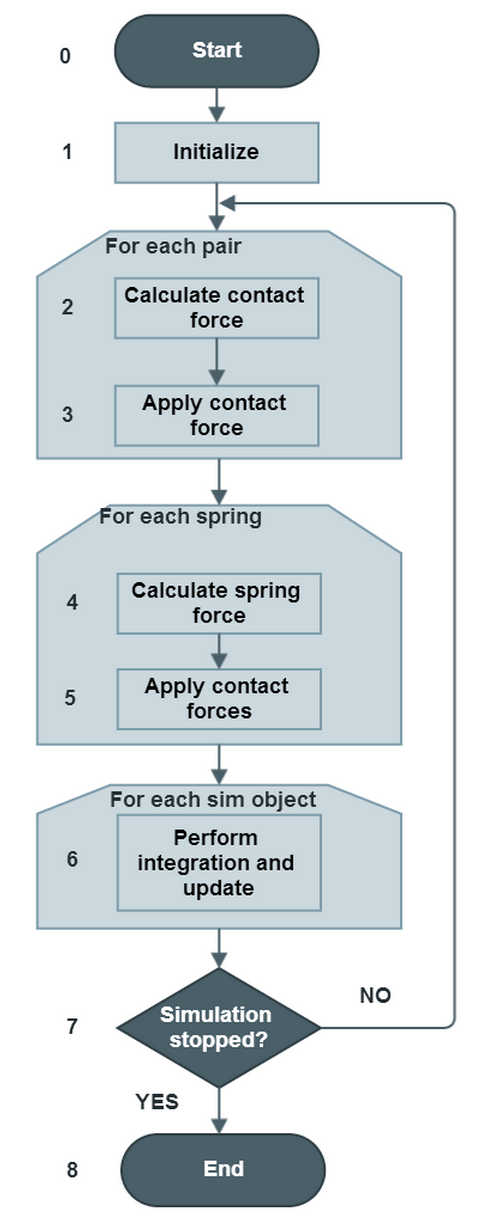
\includegraphics[width=60mm]{sections/methodology/images/basic/sim-algorithm.png}
  \caption[The flow-chart of the simulation update loop.]{\label{sim-algorithm}}
\end{figure}

\begin{enumerate}

  \item The first step includes all the required initialization and pre-processing. This step is only performed once. It should be mentioned that during this stage the spring object is instantiated and is assigned with two attachments. The attachments are represented by the attached dynamic objects’ references.

  \item Step two involves complex processing of the geometries and collision detection. This step consists of a loop going through all the simulation objects and pairwise collision detection. The calculated contact information is used to compute the resulting contact force for each contact.

  \item Steps 3 and 5 represent the same process of force and moment accumulation. For the linear component the application is a simple addition. It should be noted that the same process is used for contact and spring force application, which contributes towards a more generic physics engine and conforms with the Don’t Repeat Yourself (DRY) principle.

  \begin{equation}
  \label{eq-force-sum}
  F_{all} = \sum_{i=0}^{n}F_{n}
  \end{equation}

  \begin{equation}
  \label{eq-moments-sum}
  M_{all} = \sum_{i=0}^{n}F_{n} \times  r_{n}
  \end{equation}


  \item The fourth step involves calculating the spring force acting on the attached objects. The force is calculated according to the Hooke’s law.

  \item The resulting spring force is applied to the object in the exact same way as described in item 3. Additionally, according to Newton’s third law of motion, the inverted force is also applied to the second object.

\end{enumerate}


\subsubsection{Full Fetal Body Simulation}

The next step in developing a childbirth simulation system was including the full articulated fetal body.
Following the simplified physics modeling approach described before, we developed a spring mass model capable of representing the fetal body to some degree accuracy. The spring mass model consists of the primitives comprising the main sections of the fetal body and a number of springs that connect them. Figure \ref{full-articulated} demonstrates the sample assembly of the fetal body components.

\begin{figure}
  \centering
    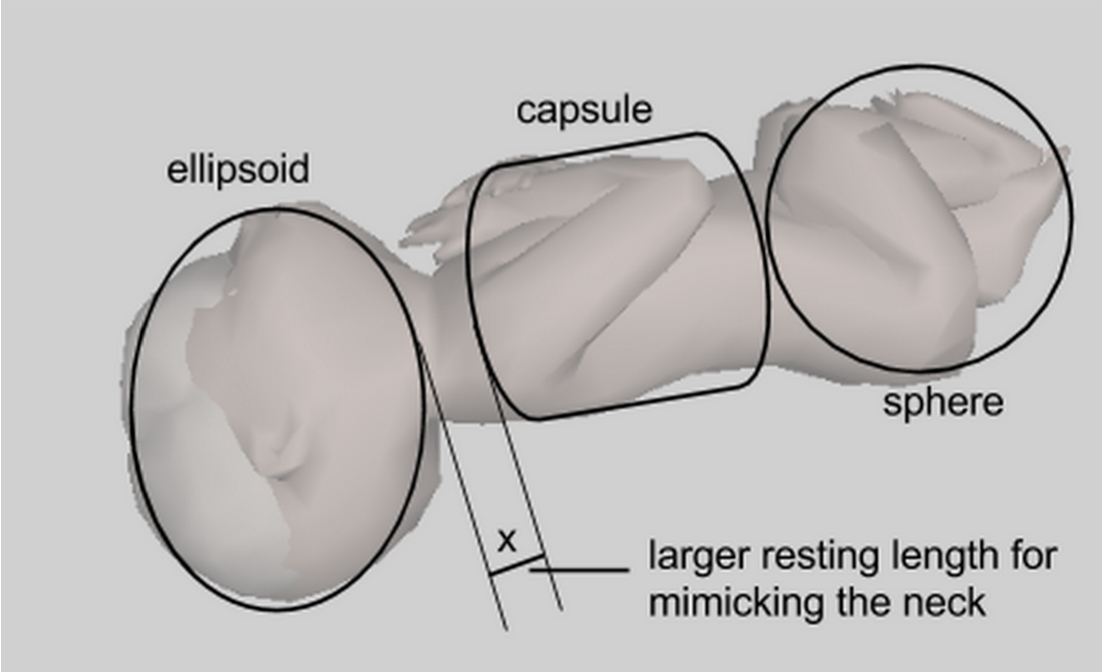
\includegraphics[width=60mm]{sections/methodology/images/basic/full-articulated.png}
  \caption[The simplified articulated mass-spring fetal body model]{\label{full-articulated}}
\end{figure}

The mass-spring model is implemented using simple Hookean springs. The forces exerted by the spring onto the bodies that it is connected to is calculated according to Hook's law \ref{eq-hooks-law}.


\begin{equation}
\label{eq-hooks-law}
F = - k * x
\end{equation}

Figure \ref{mass-spring-detail} demonstrates in detail how the forces are calculated. Two bodies $A$ and $B$ are connected by a spring with resting (relaxed) length $L_r$. The attachment points $A_1'$ and $A_2'$ are specified in the local coordinates of the objects that the attachment is on. The world vectors $A_1$ and $A_2$ are calculated by transforming the local attachment vectors by the respective transformation matrices of the attached objects. The current length of the spring $L_s$ is defined as the length of the vector $S$, which connects the attachment points in the world space and is equal to $A_2-A_1$.Thus elongation (compression) $x$ is defined by $L_s-L_r$.

\begin{figure}
  \centering
    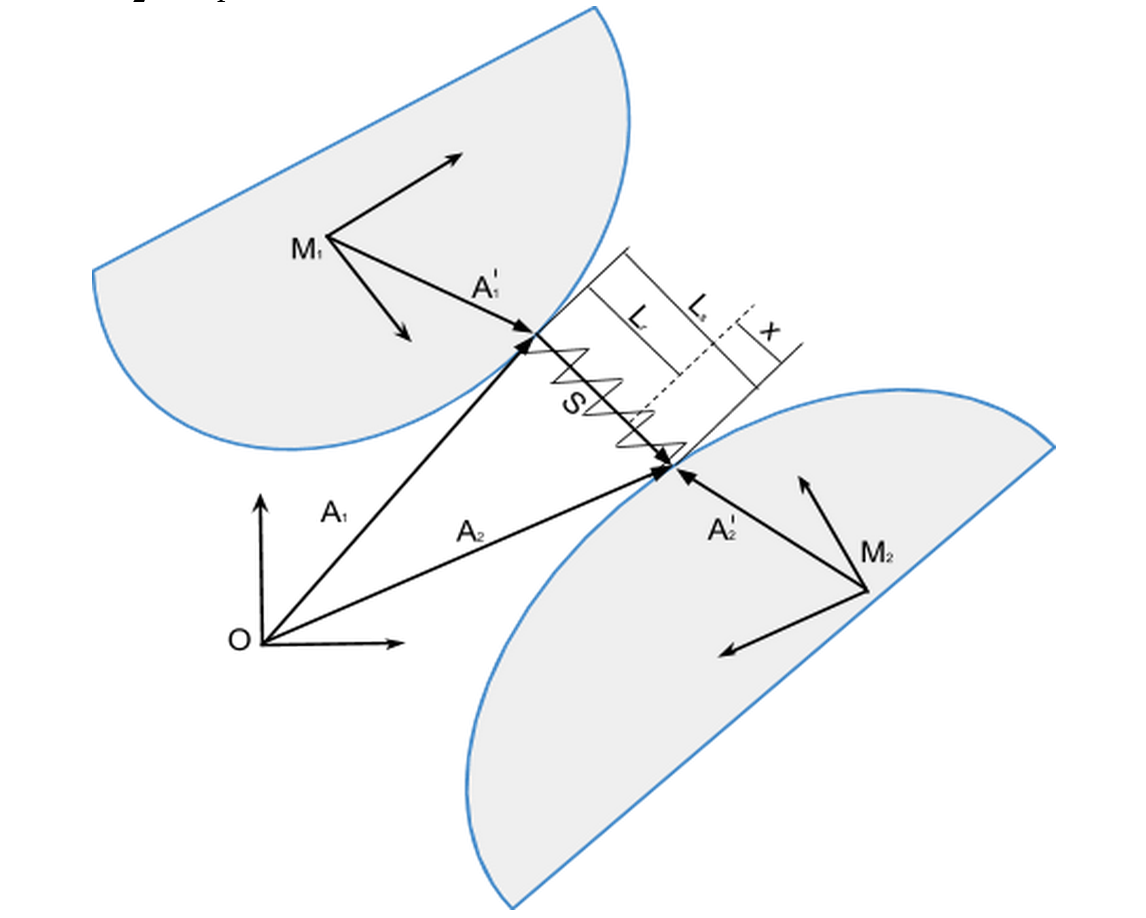
\includegraphics[width=80mm]{sections/methodology/images/basic/mass-spring-detail.png}
  \caption[The detailed representation of a single spring attachment in the full body fetal mass-spring model. ]{\label{mass-spring-detail}}
\end{figure}

\subsubsection{Results and Conclusions}

The results of the expermients performed using the described simulation system are described in the published paper \cite{gerikhanov2013}, which is also included in the appendix \ref{appendix}.

The simulation system was successful on displaying the first three cardinal movemenets. The Engagement, Descent and Flexion were observed in all experiments. As reported by the paper, the Internal Rotation was observed occasionally in cases when the flexion was manually imposed onto the fetal head. When using the hybrid approach, the simulation demonstrated all of the cardinal movements in cases when the number of way-points was sufficient to impose the required trajectory.

Using the simplified full fetal body model did not improve the simulation results. No additional cardinal movements were observed when using the simplified model, but the originally displayed movements were slightly emphasized.

The table \ref{hybrid-table} summarizes the described experimental resuts.

% !!! TABLE

\begin{table}[h]
\begin{tabular}{|l|l|l|l|l|}
\hline
\multirow{2}{*}{Cardinal movement} & \multicolumn{4}{l|}{Waypoints} \\ \cline{2-5}
                                   & 0      & 1     & 2     & 3     \\ \hline
Descent                            & +      & +     & +     & +     \\ \hline
Engagement                         & +      & +     & +     & +     \\ \hline
Flexion                            & +      & +     & +     & +     \\ \hline
Internal rotation                  & ?      & +     & +     & +     \\ \hline
Extension                          &        &       & +     & +     \\ \hline
External rotation                  &        &       &       & +     \\ \hline
Expulsion                          &        &       & +     & +     \\ \hline
\end{tabular}
\caption{Initial exerimental results} \label{hybrid-table}
\end{table}

This simplified forwards-engineered childbirth simulation system is incomplete and requires further development and refinement. This was indeed anticipated as  developing a medical simulation software with full functionality can take several years. The resulting system can be seen as an initial step towards a fully functional system for childbirth simulation and obstetrician training. The following sections describe the steps taken in order to improve upon the described simulation system.
